\begin{figure}[t]
    \centering
    % TikZ figure showing the relations between all components of the erasure codes tester

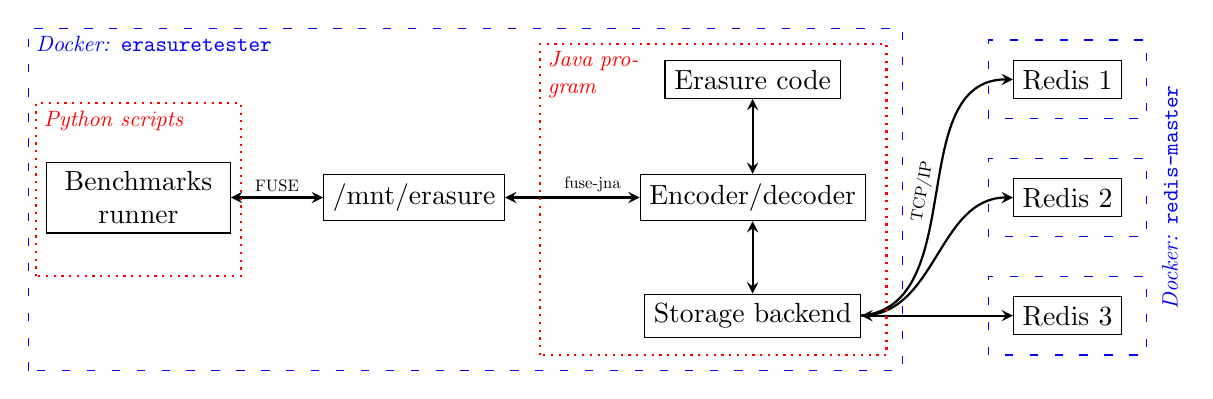
\begin{tikzpicture}
\node[draw, text width=2.1cm, text centered] (bench) at (1.2, 1.5) {Benchmarks runner};
\node[draw] (dir) at (4.7, 1.5) {/mnt/erasure};
\node[draw] (fed) at (9, 1.5) {Encoder/decoder};
\node[draw] (sb) at (9, 0) {Storage backend};
\node[draw] (ec) at (9, 3) {Erasure code};
\node[draw] (r1) at (13, 3) {Redis 1};
\node[draw] (r2) at (13, 1.5) {Redis 2};
\node[draw] (r3) at (13, 0) {Redis 3};

\draw[<->,thick,>=stealth] (bench) -- (dir) node[midway,above,scale=0.6]{FUSE};
\draw[<->,thick,>=stealth] (dir) -- (fed) node[pos=0.65,above,scale=0.6]{fuse-jna};
\draw[<->,thick,>=stealth] (fed) -- (ec);
\draw[<->,thick,>=stealth] (fed) -- (sb);
\draw[->,thick,>=stealth] (sb.east) to[out=5,in=180] node[sloped,midway,scale=0.6,above]{TCP/IP} (r1.west);
\draw[->,thick,>=stealth,out=0,in=180] (sb.east) to[out=0,in=180] (r2.west);
\draw[<->,thick,>=stealth] (sb.east) -- (r3.west);

\draw[loosely dashed,blue] (-0.2,-0.7) rectangle (10.9,3.65);
\draw[loosely dashed,blue] (12,2.5) rectangle (14,3.5);
\draw[loosely dashed,blue] (12,1) rectangle (14,2);
\draw[loosely dashed,blue] (12,-0.5) rectangle (14,0.5);
\draw[dotted,red,thick] (6.3,-0.5) rectangle (10.7,3.45);
\draw[dotted,red,thick] (-0.1,0.5) rectangle (2.5,2.7);

\draw (6.3,3.45) node[below right,red,scale=0.8, text width=1.5cm] {\textit{Java program}};
\draw (-0.1,2.7) node[below right,red,scale=0.8] {\textit{Python scripts}};
\draw (-0.2,3.65) node[below right,blue,scale=0.8] {\textit{Docker:} \texttt{erasuretester}};
\draw (14.3,1.5) node[blue,scale=0.8,rotate=90] {\textit{Docker:} \texttt{redis-master}};
\end{tikzpicture}

    \caption{Architecture of ErasureBench.}
    \label{fig:architecture}
\end{figure}

\section{The ErasureBench Framework}
\label{sec:erasure-tester}

The ErasureBench framework allows researchers to easily evaluate the performances of erasure codes when used in a large-scale storage context.
It exposes a filesystem interface to the end-user to facilitate the adoption of well-known file-system benchmarks.\footnote{Due to the lack of space, we omit experiments using tools such as IOzone or FileBench.}
Files are processed (encoded), split into blocks and stored in a key-value store.
Thanks to its decoupled architecture, each of the three components (filesystem interface, key-value store, erasure code implementation) can be easily replaced by alternative implementations. 
In the remainder of this section we provide further details about the software architecture and our implementation choices.
%While the Java program can be used standalone, it is designed to run in a Docker container shared with associated Python scripts.

\textbf{Architecture.} \autoref{fig:architecture} depicts the architecture of ErasureBench.
At its core, ErasureBench exposes a filesystem interface via a Linux mount point implemented via \ac{fuse}. 
Upon its execution, the filesystem is mounted under a regular directory. 
Low-level IO system calls are intercepted by the \textit{fuse-jna}\footnote{\url{https://github.com/EtiennePerot/fuse-jna}} Java library.
The blocks are then sent back and forth to the encoder/decoder layer. 
The encoder/decoder first chunks data in blocks of the chosen size and aligns read and write operations to the correct boundaries\vs{which ones?}. 
Once chunked, blocks are  processed by the chosen erasure code to generate the redundancy blocks. 
Finally, data and parity blocks are passed to the storage backend.

\begin{figure}[t]
    \centering
    % TikZ figure showing how blocks are splitted and encoded

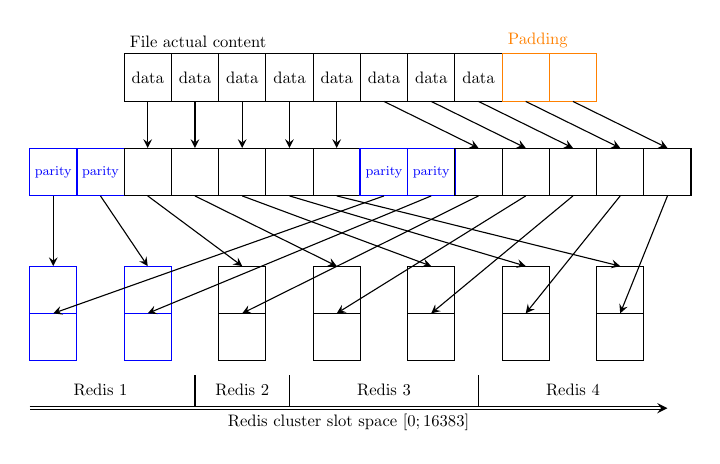
\begin{tikzpicture}[transform shape,scale=0.6]
\draw (1.5,0.5) node[above right] {File actual content};
\node (d1) at (2,0) [draw,minimum width=1cm,minimum height=1cm] {data};
\node (d2) at (3,0) [draw,minimum width=1cm,minimum height=1cm] {data};
\node (d3) at (4,0) [draw,minimum width=1cm,minimum height=1cm] {data};
\node (d4) at (5,0) [draw,minimum width=1cm,minimum height=1cm] {data};
\node (d5) at (6,0) [draw,minimum width=1cm,minimum height=1cm] {data};
\node (d6) at (7,0) [draw,minimum width=1cm,minimum height=1cm] {data};
\node (d7) at (8,0) [draw,minimum width=1cm,minimum height=1cm] {data};
\node (d8) at (9,0) [draw,minimum width=1cm,minimum height=1cm] {data};
\draw (9.5,0.5) node[above right,orange] {Padding};
\node (d9) at (10,0) [orange,draw,minimum width=1cm,minimum height=1cm] {};
\node (d10) at (11,0) [orange,draw,minimum width=1cm,minimum height=1cm] {};

\node (p1) at (0,-2) [draw,minimum width=1cm,minimum height=1cm,blue] {\footnotesize parity};
\node (p2) at (1,-2) [draw,minimum width=1cm,minimum height=1cm,blue] {\footnotesize parity};
\node (p3) at (2,-2) [draw,minimum width=1cm,minimum height=1cm] {};
\node (p4) at (3,-2) [draw,minimum width=1cm,minimum height=1cm] {};
\node (p5) at (4,-2) [draw,minimum width=1cm,minimum height=1cm] {};
\node (p6) at (5,-2) [draw,minimum width=1cm,minimum height=1cm] {};
\node (p7) at (6,-2) [draw,minimum width=1cm,minimum height=1cm] {};
\node (p8) at (7,-2) [draw,minimum width=1cm,minimum height=1cm,blue] {\footnotesize parity};
\node (p9) at (8,-2) [draw,minimum width=1cm,minimum height=1cm,blue] {\footnotesize parity};
\node (p10) at (9,-2) [draw,minimum width=1cm,minimum height=1cm] {};
\node (p11) at (10,-2) [draw,minimum width=1cm,minimum height=1cm] {};
\node (p12) at (11,-2) [draw,minimum width=1cm,minimum height=1cm] {};
\node (p13) at (12,-2) [draw,minimum width=1cm,minimum height=1cm] {};
\node (p14) at (13,-2) [draw,minimum width=1cm,minimum height=1cm] {};

\draw[->,>=stealth] (d1.south) to (p3.north);
\draw[->,>=stealth] (d2.south) to (p4.north);
\draw[->,>=stealth] (d3.south) to (p5.north);
\draw[->,>=stealth] (d4.south) to (p6.north);
\draw[->,>=stealth] (d5.south) to (p7.north);
\draw[->,>=stealth] (d6.south) to (p10.north);
\draw[->,>=stealth] (d7.south) to (p11.north);
\draw[->,>=stealth] (d8.south) to (p12.north);
\draw[->,>=stealth] (d9.south) to (p13.north);
\draw[->,>=stealth] (d10.south) to (p14.north);

\node (r1) at (0,-4.5) [blue,draw,minimum width=1cm,minimum height=1cm] {};
\node (r2) at (2,-4.5) [blue,draw,minimum width=1cm,minimum height=1cm] {};
\node (r3) at (4,-4.5) [draw,minimum width=1cm,minimum height=1cm] {};
\node (r4) at (6,-4.5) [draw,minimum width=1cm,minimum height=1cm] {};
\node (r5) at (8,-4.5) [draw,minimum width=1cm,minimum height=1cm] {};
\node (r6) at (10,-4.5) [draw,minimum width=1cm,minimum height=1cm] {};
\node (r7) at (12,-4.5) [draw,minimum width=1cm,minimum height=1cm] {};

\node (r8) at (0,-5.5) [blue,draw,minimum width=1cm,minimum height=1cm] {};
\node (r9) at (2,-5.5) [blue,draw,minimum width=1cm,minimum height=1cm] {};
\node (r10) at (4,-5.5) [draw,minimum width=1cm,minimum height=1cm] {};
\node (r11) at (6,-5.5) [draw,minimum width=1cm,minimum height=1cm] {};
\node (r12) at (8,-5.5) [draw,minimum width=1cm,minimum height=1cm] {};
\node (r13) at (10,-5.5) [draw,minimum width=1cm,minimum height=1cm] {};
\node (r14) at (12,-5.5) [draw,minimum width=1cm,minimum height=1cm] {};


\draw[->,>=stealth] (p1.south) to (r1.north);
\draw[->,>=stealth] (p2.south) to (r2.north);
\draw[->,>=stealth] (p3.south) to (r3.north);
\draw[->,>=stealth] (p4.south) to (r4.north);
\draw[->,>=stealth] (p5.south) to (r5.north);
\draw[->,>=stealth] (p6.south) to (r6.north);
\draw[->,>=stealth] (p7.south) to (r7.north);
\draw[->,>=stealth] (p8.south) to (r8.north);
\draw[->,>=stealth] (p9.south) to (r9.north);
\draw[->,>=stealth] (p10.south) to (r10.north);
\draw[->,>=stealth] (p11.south) to (r11.north);
\draw[->,>=stealth] (p12.south) to (r12.north);
\draw[->,>=stealth] (p13.south) to (r13.north);
\draw[->,>=stealth] (p14.south) to (r14.north);

\node (redis1) at (1,-6.6) {Redis 1};
\draw (3,-6.3) to (3,-6.95);
\node (redis1) at (4,-6.6) {Redis 2};
\draw (5,-6.3) to (5,-6.95);
\node (redis1) at (7,-6.6) {Redis 3};
\draw (9,-6.3) to (9,-6.95);
\node (redis1) at (11,-6.6) {Redis 4};
\draw[->,>=stealth,double] (-0.5,-7) to node[midway,below]{Redis cluster slot space $\left[0;16383\right]$} (13,-7);

\end{tikzpicture}

    \caption{Splitting file contents in blocks, applying erasure coding, and storing data and parity blocks in a Redis cluster.}
    \label{fig:blocks}
\end{figure}

%\hm{The part that follows is standard. We can cut there is space is missing.}
\textbf{Blocks storage.} The storage backend is designed to operate on 1 byte blocks. 
As usual, storing each block individually in the key-value store is a very slow operation: the metadata is much bigger than the data itself, leading to unworkable overheads. 
We therefore added an intermediate layer between the encoder/decoder and the storage backend. 
This layer is transparent to the encoder/decoder which still deals with single 1 byte blocks. 
Thanks to this new layer, we aggregate multiple write operations on the key-value store, and each key stores an aggregation of multiple blocks.
The guarantees offered by the erasure coding process are still kept because one aggregation only stores blocks that belong to the same stripe position. 
This additional component provides a considerable speed-up comprised between $100\times$ and $1000\times$. 
\autoref{fig:blocks} shows how files are split in blocks, erasure coded, and then aggregated and stored on multiple Redis servers. %\hm{The aggregation is not clear in the figure. Valerio, could you improve it?}
A \ac{lru} cache optimizes the retrieval of multiple individuals blocks.
This way, when reading a file sequentially, each block aggregation is only retrieved once from the key-value store.

\textbf{Metadata management.} We keep track of the location of each stored block. 
Our strategy is to assign a 32-bit key to each block. 
From each key, we can infer two related identifiers: a Redis key and an offset. 
The Redis key points to an aggregation of blocks stored in the Redis cluster. 
We then use the offset to precisely locate the block we want within the aggregation.
In the current prototype, we store all metadata in memory. 
Each file consists in a list of identifiers. 
We also store the size of the file once decoded to discard padding blocks. 
%Naturally, the space overhead of our solution is important, so ErasureBench is not able to store a large amount of data.

\textbf{Implementation details.}
%The frontend has one available implementation: a \ac{fuse} filesystem interface backed by \textit{fuse-jna} \autocite{fuse-jna}.
%The encoder/decoder layer is not modular because it is sufficient to have one correct way of handling that operation. 
We implement the erasure coding algorithms described in Section~\ref{sec:codes} and we bundled them in ErasureBench. 
We extracted and adapted the \ac{lrc} libraries from \autocite{XorbasVLDB} to remove dependencies on any other \textit{Hadoop} component. 
%In addition, an additional code taking two data blocks and generating a single parity block by xoring them is also inherited from~\autocite{XorbasVLDB} and thus available. \hm{Please confirm this last code. We have no simulations for it.}
%A fourth algorithm is provided, in the name of the \textit{Null} encoder.
%As its name suggests, its \textit{modus operandi} consists in simply forwarding data blocks without any added redundancy.
%Failing to read a data block while using the \textit{Null} encoder signifies the loss of the stripe associated with it.
We use the Redis distributed key-value store\footnote{\url{http://redis.io}} via the efficient and battle-tested \textit{Jedis}  binding.\footnote{\url{https://github.com/xetorthio/jedis}}
For testing purposes, an in-memory storage backend is also available.

\textbf{Deployment.} The deployment of ErasureBench requires to simultaneously launch multiple independent services and to coordinate their bootstrap. 
%On top of these services, we want to perform measurements on the performance of different erasure coding libraries. 
We leverage the Docker\footnote{\url{https://www.docker.com}} technology to facilitate this task.
We also exploit Docker Swarm\footnote{\url{https://docs.docker.com/swarm/}} to reduce as much as possible the deployment differences between a local and a remote cluster setup. % to run the benchmarks on a local machine or on a cluster of machines is similar. 
All the components as well as the supporting Python scripts are packaged as Docker images.
The framework allows to easily parametrize the testbed (size of the cluster, erasure code and associated parameters, etc.) by means of configuration files. 
We further provide Python scripts to setup all the components, execute the benchmarks and collect the resulting logs.
%When an experimenter wants to start the benchmarks with, say, a 20-node Redis cluster as storage backend, he/she only needs to specify the desired setup in a configuration file.
%The supporting Python scripts will configure the Redis cluster, run the benchmarks and collect the results. 
We use the Redis's own \texttt{redis-trib.rb} script\footnote{\url{http://download.redis.io/redis-stable/src/redis-trib.rb}} to initialize the storage cluster.
However we observed severe performance issues with cluster sizes bigger than few dozens.
Therefore, we implemented similar logics in our own Python scripts in order to scale the cluster faster.
%We can also use \textit{redis-trib.rb} to scale the cluster, but it is rather slow with more than a dozen nodes. 
%We instead implemented the same logic in our own Python scripts in order scale the cluster faster.
%Thanks to Docker Swarm, the setup to run the benchmarks on a local machine or on a cluster of machines is similar. 
%The system can use any reasonable number of Redis servers. 
ErasureBench includes shell scripts that automate the complete pipeline, from the compilation of sources to the execution of benchmarks on a remote Docker Swarm cluster.

\textbf{Fault injection.}
ErasureBench supports the injection of synthetic and real failure traces. 
A synthetic trace is simply a list of system sizes: when a benchmark completes an iteration, we resize the storage cluster using the next value in the list. 
ErasureBench can inject real failure traces stored in a SQLite database in the format described in \autocite{fta-journal}. 
These traces monitor individual nodes of a real-life distributed system and record failure events in a database. 
ErasureBench can replay these traces to replicate a real-world failure pattern by first creating a storage cluster of the same size as the original system. 
New nodes are instantiated and old nodes killed at the same rates as reported in the trace. 
Finally, the framework allow to restrict the replay to a limited time interval of the trace.
We use this trace replay feature in the last set of experiments in the next section.